\documentclass{article}

\usepackage{amsmath}
\usepackage{xfrac}
\usepackage{bbm}
\usepackage{multicol}
\usepackage{geometry}
\usepackage{multirow}
\geometry{margin=1in}

\providecommand{\e}[1]{\ensuremath{\times 10^{#1}}}

\title{F100-PW-220 Engine Model}
\author{Richard W. Fenrich\\Department of Aeronautics and Astronautics\\Stanford University, Stanford, CA\\rfenrich@stanford.edu}
\date{July 31, 2015}

\begin{document}

\maketitle

%\section*{Nomenclature}
%
%\begin{multicols}{2}
%\begin{tabbing}
%  XXX \= \kill% this line sets tab stop
%  $A$ \> local cross-sectional area \\
%  $C_f$ \> local skin friction coefficient \\
%  $C_p$ \> specific heat capacity, const. $P$ \\
%  $D$ \> local diameter of nozzle \\
%  $f(M)$ \> area-Mach function \\
%  $h$ \> heat transfer coefficient \\
%  $k$ \> thermal conductivity \\
%  $M$ \> local Mach number \\  
%  $Nu$ \> Nusselt number \\
%  $P$ \> pressure \\
%  $Pr$ \> Prandtl number \\
%  $\dot{Q}$ \> transverse outward heat flow \\
%  $R$ \> thermal resistance \\
%  $Re$ \> Reynolds number \\
%  $S$ \> Sutherland coefficient \\
%  $T$ \> temperature \\
%  $t$ \> wall thickness \\
%  $U$ \> velocity \\
%  $x$ \> distance along nozzle axis \\
%  $\gamma$ \> ratio of specific heats \\ 
%  $\mu$ \> dynamic viscosity \\
%  $\rho$ \> density \\
%  $\sigma$ \> hoop stress \\
%  \\
%  \textit{Subscript}\\
%  $f$ \> fluid \\
%  $i$ \> incompressible \\
%  $t$ \> stagnation property \\
%  $w$ \> nozzle wall \\  
%  $x$ \> based on x \\
%  $\infty$ \> environment \\
%  \textit{Superscript}\\
%  $*$ \> sonic condition \\
%  $'$ \> reference \\
% \end{tabbing}
% \end{multicols}

\section{Introduction}

The F100-PW-220 after-burning turbofan engine is considered to be the most reliable military turbofan engine in the world. Its predecessors were the F100-100 and F100-200 engines, respectively. Pratt \& Whitney released the upgraded F100-PW-220 engine in 1985, which fixed previous reliance and maintenance issues. A more powerful version of the engine, the F100-PW-229 was released in 1991.

\begin{figure}
\caption{F100-PW-220 illustration from Pratt \& Whitney}
\label{fig:engine_illustration}
\begin{center}
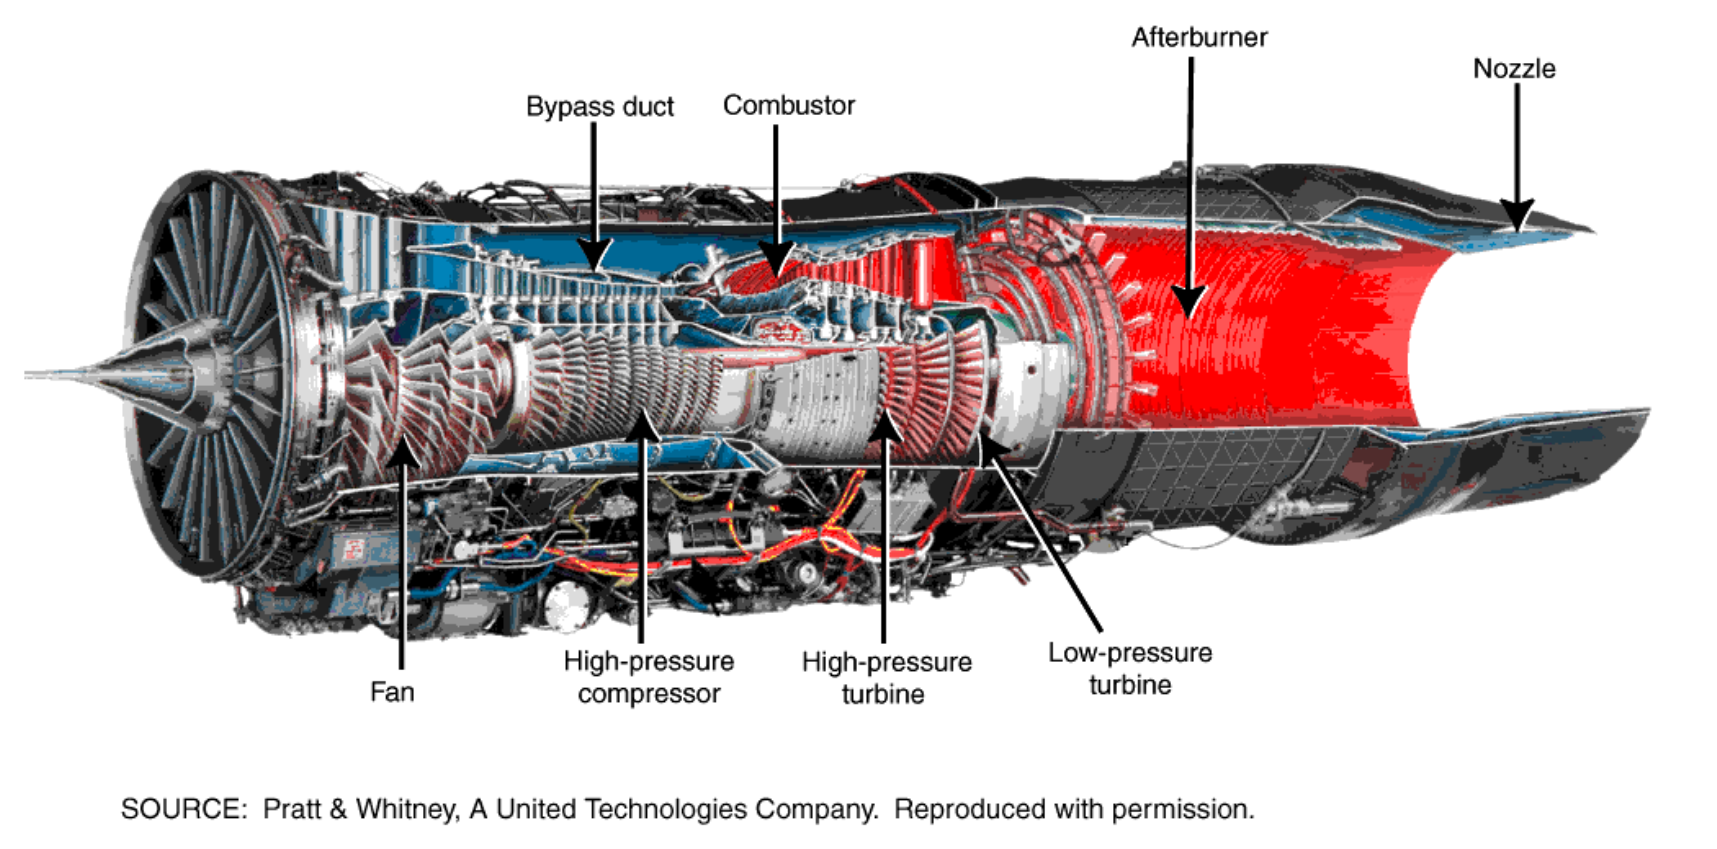
\includegraphics[scale=0.5]{figs/F100-PW-220-Military_Jet_Acquisition_by_RAND_Project_Air_Force.png}
\end{center}
\end{figure}

Today, the F100-PW-220 and F100-PW-229 engines power all F-15E jets. In addition, the F100-PW-220 engine was chosen to power Northrop Grumman's unmanned combat vehicle, the X-47B, without after-burning capabilities. The focus of this current research is on developing a simplified nozzle model for aircraft such as the X-47B, which can be used for uncertainty quantification and design under uncertainty. Due to the interaction between the nozzle and the rest of the turbofan engine, it is necessary to develop a simplified model of the F100-PW-220 engine for more detailed nozzle analysis. The following report details the nature of this model.

\subsection{Specifications}

\subsubsection{X-47B}
Table \ref{tab:x47b_specifications} summarizes the geometry and estimated performance of the X-47B.

\begin{table}
\caption{X-47B specifications}
\label{tab:x47b_specifications}
\begin{center}
\begin{tabular}[]{c | c }
Parameter & Value \\
\hline
Span (m) & 18.93 \\
Empty weight (kg) & 6,350 \\
TOGW (kg) & 20,215 \\
Payload (kg) & 2,040 \\
 $\textrm{L/D}_{\textrm{cruise}}$* & 12.62 - 15.58 \\
Cruise Mach* & 0.45 \\
Top Speed & high subsonic \\
Range (nm) & 2,100 \\
Endurance (hr) & 6 \\
Service Ceiling (ft) & 40,000 \\
\end{tabular} \\
\footnotesize{*from Virginia Tech student report}
\end{center}
\end{table}

\subsubsection{F100-PW-220}

Performance and geometric data of the F100-PW-220 engine is sparse. Nevertheless, Table \ref{tab:engine_specifications} presents a summary of performance and geometric data obtained from various sources.

\begin{table}
\caption{F100-PW-220 specifications from literature}
\label{tab:engine_specifications}
\begin{center}
\begin{tabular}[]{c | c }
Parameter & Value \\
\hline
Bypass ratio & 0.6 \\
Length* (m) & 4.855 \\
Inlet diameter (m) & 0.884 \\
Fan diameter (m) & 0.928 \\
Max diameter (m) & 1.181 \\
Max thrust - dry (N) & 64,900 \\
Max thrust* (N) & 105,720 \\
sfc (lb/lbf/hr) & 0.73 \\
max sfc (lb/lbf/hr)* & 2.1 \\
Fan pressure ratio & 3.06 \\
Overall pressure ratio & 24.5 \\
Turbine inlet temp. (K) & 1672.15 \\
Air flow (kg/s) & 101.6-103.4 \\
Dry weight (N) & 14,530 \\
\end{tabular} \\
\footnotesize{*with afterburner}
\end{center}
\end{table}

\subsection{Operation}

The F100-PW-220 engine uses a full-authority digital electronic engine control (DEEC) system \cite{Childre1989}. In its basic control mode, the DEEC uses the gas generator fuel flow to control the fan operating point, and uses the exhaust nozzle area to control the engine overall pressure ratio (stagnation pressure ratio from compressor exit to fan inlet). However, the DEEC responds to approximately 50 input parameters and can use up to about 20 outputs to control the engine \cite{Childre1989}.


\section{Model}

A schematic of a generic military turbofan engine is presented in Figure \ref{fig:turbofan_schematic}. 

\begin{figure}
\caption{Schematic of military turbofan engine \cite{cantwell283}}
\label{fig:turbofan_schematic}
\begin{center}
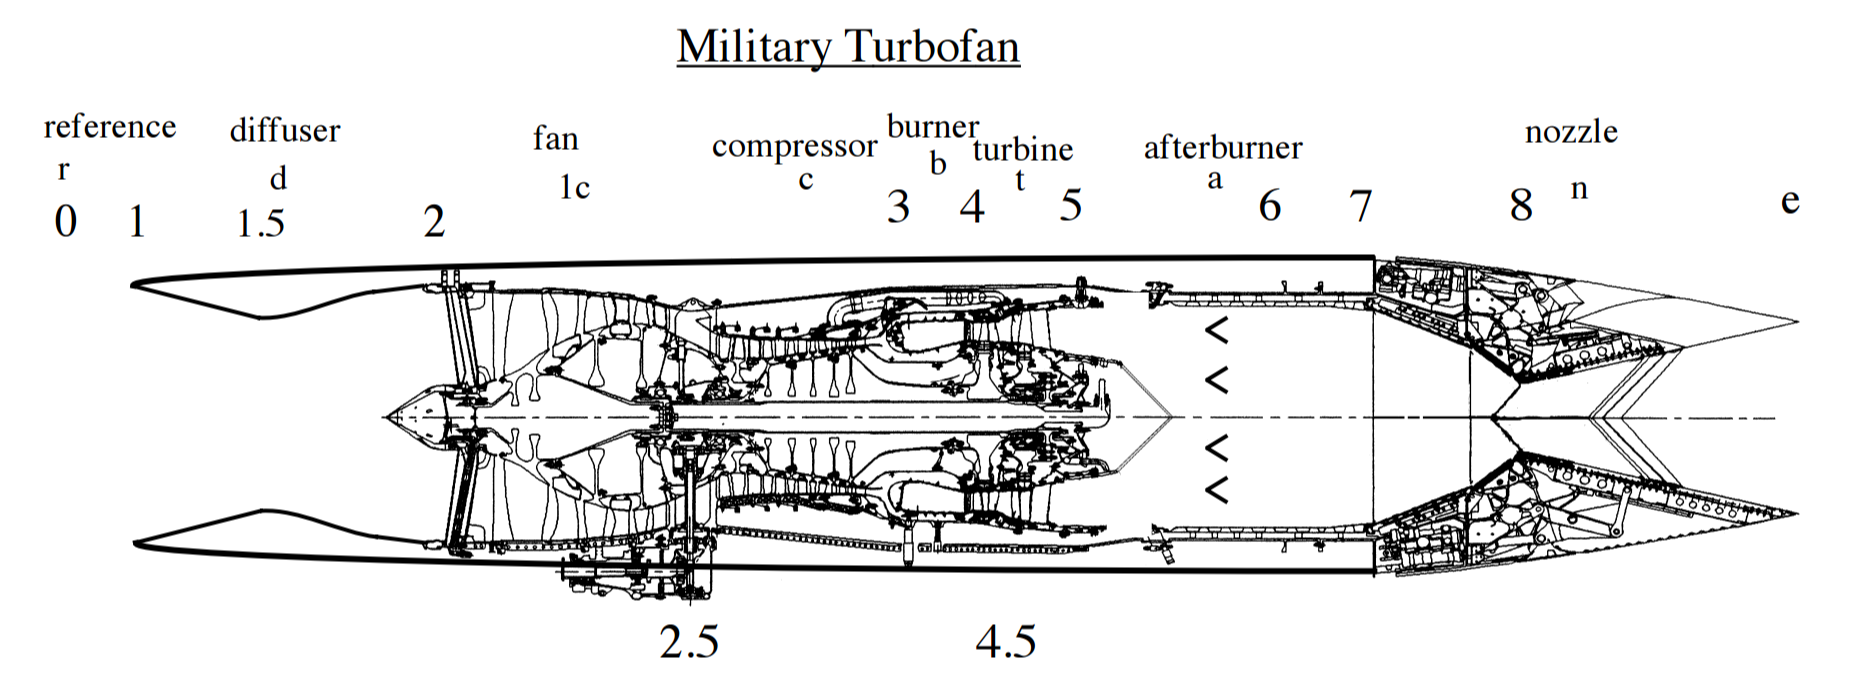
\includegraphics[scale=0.4]{figs/Military_Turbofan_Schematic_Cantwell.png}
\end{center}
\end{figure}

\subsection{Notation}
Analysis is performed primarily in terms of stagnation pressure and stagnation temperature ratios, denoted by $\pi$ and $\tau$, respectively. Subscripts are used to denote engine components, and numbers used to denote engine stations. For example, $\sfrac{P_{t3}}{P_{t2.5}}$, the stagnation pressure ratio across the compressor is denoted by $\pi_c$. The only exception to this rule is $\pi_r = \sfrac	{P_{t\infty}}{P_{\infty}}$ which is the ratio of a stagnation to a static pressure. Note that the subscript $t$ which is used to denote stagnation quantities is also used to denote the turbine.

\subsection{Equations}

Analysis of the turbofan engine begins with splitting the engine into its respective components, and then applying the area-averaged equations of motion (equations \ref{eq:equation_of_motion1}, \ref{eq:equation_of_motion2}, \ref{eq:equation_of_motion3}) starting from the nozzle and working forwards \cite{cantwell283}. 

\begin{gather}
\label{eq:equation_of_motion1}
d(\rho U) = \frac{\delta \dot{m}}{A} - \rho U \frac{dA}{A} \\
\label{eq:equation_of_motion2}
d(P - \tau_{xx}) = \rho U dU = - \frac{1}{2} \rho U^2 \left( 4 C_f \frac{dx}{D} \right) + \frac{(U_{xm} - U) \delta \dot{m}}{A} - \frac{\delta F_x}{A} \\
\label{eq:equation_of_motion3}
d \left( h_t - \frac{\tau_{xx}}{\rho} + \frac{Q_x}{\rho U} \right) = \delta q - \delta w + \left( h_{tm} - \left	( h_t - \frac{\tau_{xx}}{\rho} + \frac{Q_x}{\rho U} \right) \right) \frac{\delta \dot{m}}{\rho U A}
\end{gather}

The above equations can be manipulated in terms of stagnation temperature and pressure, and Mach number. In addition, a useful relation for analyzing aircraft engines is the following mass conservation relationship \cite{cantwell283}:

\begin{equation}
\label{eq:mdot}
\dot{m} = \rho U A = \frac{\gamma}{\left( \frac{\gamma + 1}{2} \right)^{ \frac{\gamma + 1}{2 (\gamma - 1)}}} \left( \frac{P_t A}{\sqrt{ \gamma R T_t}} \right) f(M)
\end{equation}

\begin{equation}
\label{eq:area_mach_function}
f(M) = \frac{A^*}{A} = \left( \frac{\gamma + 1}{2} \right)^{\frac{\gamma + 1}{2 (\gamma + 1)}} \left( \frac{M}{\left( 1 + \frac{\gamma -1}{2} M^2 \right)^{\frac{\gamma + 1}{2 (\gamma - 1)}}}\right)
\end{equation}

Assume negligible friction, external axial force, and heat transfer throughout the engine. Thus:

\begin{equation*}
C_f = \delta F_x = \delta q = 0
\end{equation*}

Also assume streamwise normal stresses $\tau_{xx}$ and heat fluxes $Q_x$ can be neglected. It is common to assume an ideal diffuser and nozzle, with an isentropic fan, compressor, and turbine, and negligible stagnation pressure losses across the burner. However, in our efforts, we aim to model the non-ideal turbofan engine.

\subsection{Component Analysis}

In the following analysis several convenient ratios are used. These include the bypass ratio $\beta$:

\begin{equation*}
\beta = \frac{\dot{m}_{\beta}}{\dot{m}_c}
\end{equation*}

and the fuel mass flow fraction $f$:

\begin{equation*}
f = \frac{\dot{m}_f}{\left( \dot{m}_c + \dot{m}_{\beta} \right)}
\end{equation*}

\subsubsection{Freestream}
Freestream conditions are given, allowing stagnation temperature and pressure to be easily calculated.

\subsubsection{Diffuser}
Realistic stagnation pressure and temperature ratios are assigned to the diffuser \textit{a priori}.

\subsubsection{Fan}
The fan stagnation pressure ratio $\pi_f$ is given. The stagnation temperature ratio can be estimated, taking into account the polytropic efficiency of the fan\footnote{Note that the isentropic efficiency of the fan can be calculated from the polytropic efficiency of the fan at a given stagnation pressure ratio.} of the fan:

\begin{equation*}
\tau_f = \pi_f^{\frac{\gamma-1}{\gamma \eta_{p,f}}}
\end{equation*}

The fan bypass duct ignores any heat transfer from the burner and also ignores stagnation pressure losses.

\subsubsection{Compressor}
The overall pressure ratio, defined as the ratio of the compressor exit stagnation pressure to the fan inlet stagnation pressure, is known. Thus, the stagnation pressure ratio across the compressor only can be calculated as:

\begin{equation*}
\pi_c = \frac{\pi_{\textrm{overall}}}{\pi_r \pi_d \pi_f}
\end{equation*}

The stagnation temperature ratio across the compressor can be estimated by taking into account the polytropic efficiency of the compressor:

\begin{equation*}
\tau_c = \pi_c^{\frac{\gamma-1}{\gamma \eta_{p,c}}}
\end{equation*}

Then the overall stagnation temperature ratio can be calculated from fan and compressor stagnation temperature ratios:

\begin{equation*}
\tau_{\textrm{overall}} = \tau_c \tau_f
\end{equation*}

\subsubsection{Burner}
A burner stagnation pressure ratio $\pi_b$ is assumed. The turbine inlet temperature $T_{t5}$ is known for the F100-PW-220, so the stagnation temperature ratio can be calculated as:

\begin{equation*}
\tau_b = \frac{T_{t5}}{T_{t4}}
\end{equation*}

\subsubsection{Fuel Flow}

Using conservation of energy on a control volume surrounding the burner with burner efficiency $\eta_b$ gives:

\begin{equation*}
\dot{m}_f (\eta_b h_f - h_{t4}) = \dot{m}_c ( h_{t4} - h_{t3})
\end{equation*}

Divide both sides by $\dot{m}_c C_p T_{t2}$, and define the fuel-core mass flow ratio $f = \sfrac{\dot{m}_f}{\left( \dot{m}_c + \dot{m}_{\beta} \right)}$:

\begin{equation*}
f \left( \frac{\eta_b h_f}{C_p T_{t2}} - \frac{T_{t4}}{T_{t2}} \right) = \frac{1}{1 + \beta} \left( \frac{T_{t4}}{T_{t2}} - \frac{T_{t3}}{T_{t2}} \right)
\end{equation*}

Now define the following useful stagnation temperature ratio, $\tau_{\lambda}$ where $\tau_{\lambda} = \sfrac{T_{t4}}{T_{t2}}$, and solve for $f$:

\begin{equation*}
f = \frac{\tau_{\lambda} - \tau_{\textrm{overall}}}{ \left( 1 + \beta \right) \left( \frac{ \eta_b h_f}{C_p T_{t2}} - \tau_{\lambda} \right) }
\end{equation*}

If instead, $f$ is prescribed, the turbine exit stagnation temperature can be calculated from:

\begin{equation*}
\tau_{\lambda} = \frac{ f \frac{\eta_b h_f}{C_p T_{t2}} + \frac{\tau_{\textrm{overall}}}{1 + \beta}}{f + \frac{1}{1 + \beta}}
\end{equation*}

\subsubsection{Turbine}
The turbine temperature ratio can be calculated by work matching with the compressor \cite{cantwell283}. Note the addition of a shaft efficiency $\eta_m$:

\begin{equation*}
\tau_t = 1 - \frac{\tau_{\textrm{overall}} - 1 + \beta \left( \tau_f - 1 \right) }{\tau_{\lambda} \eta_m \left( 1 + f + \beta f \right)}
\end{equation*}

where $\tau_{\lambda} = \sfrac{T_{t4}}{T_{t2}}$. Stagnation pressure ratio can be calculated using an assumed polytropic efficiency factor \cite{cantwell283}:

\begin{equation*}
\pi_t = \tau_t^{\frac{\gamma}{(\gamma - 1) \eta_{pt}}}
\end{equation*}

\subsubsection{Bypass and Core Air Mixing}
\label{sec:mixing}

Both the bypass air in the fan duct and the core air exiting from the turbine enter the nozzle inlet. In keeping with the area averaged assumption already used, the static pressure and static temperature are area averaged across the nozzle inlet and used to determine the corresponding stagnation pressure and temperature. The process begins by determining the Mach numbers at the fan bypass and turbine exits. Conservation of mass yields the following relationship (see equation \ref{eq:mdot}):

\begin{equation*}
\frac{P_{t,7f} A_{7f} f \left( M_{7f} \right) }{ \sqrt{T_{t,7f}}} = \beta \frac{P_{t,7t} A_{7t} f \left( M_{7t} \right) }{ \sqrt{T_{t,7t}}}
\end{equation*}

Rearranging shows that if $M_{7f}$ is known, then $M_{7t}$ can be calculated:

\begin{equation*}
f(M_{7t}) = \frac{1}{\beta} \sqrt{\frac{T_{t,7t}}{T_{t,7f}}} \frac{P_{t,7f}}{P_{t,7t}} \frac{A_{7f}}{A_{7t}} f( M_{7f})
\end{equation*}

In practice, the Mach number at the fan bypass exit $M_{7f}$ must be assumed. However, only certain values of $M_{7f}$ will satisfy the mass conservation equation. A good estimate is between $0.4$ and $0.8$, depending on the flight regime\footnote{The current software implementation assumes a fan bypass exit Mach number $M_{7f}$ unless the user prescribes otherwise. If the mass conservation equation is not satisfied, then $M_{7f}$ will be adjusted until the it is satisfied.}. With $M_{7f}$ assumed, then $M_{7t}$ can be calculated, and static pressures and temperatures for the bypass and core flows can be calculated using the definition of the stagnation property. For example, the static temperatures can be calculated as:

\begin{gather*}
T_{7f} = \frac{T_{t,7f}}{1 + \frac{\gamma - 1}{2} M_{7f}^2} \\
T_{7t} = \frac{T_{t,7t}}{1 + \frac{\gamma - 1}{2} M_{7t}^2}
\end{gather*}

Now, the static properties can be area-averaged. Assuming the area ratio of bypass air to core air at the nozzle inlet ($\sfrac{A_{7f}}{A_{7t}}$) can be estimated, the following integral can be written:

\begin{equation}
\label{eq:T7_integral}
\begin{split}
\int T dA_7 & = \int_{\textrm{bypass}}  T_{7f} dA_{7f} + \int_{\textrm{core}} T_{7t} dA_{7t} \\
T_7 A_7 & = T_{7f} A_{7f} +T_{7t} A_{7t} \\
T_7 & = T_{7f} \frac{\sfrac{A_{7f}}{A_{7t}}}{1 + \sfrac{A_{7f}}{A_{7t}}} +T_{7t} \frac{1}{1 + \sfrac{A_{7f}}{A_{7t}}}
\end{split}
\end{equation}

An average static pressure $P_7$ can be calculated in the same manner. By also averaging the velocity ($U_7$), and using the definition of the Mach number, the Mach number at the nozzle inlet can be determined:

\begin{equation}
M_7 = \frac{U_7}{\sqrt{\gamma R T_7}} = 
\frac{ M_{7f} \sqrt{\gamma R T_{7f}} \frac{A_{7f}}{A_7}  + M_{7t} \sqrt{\gamma R T_{7t}} \frac{A_{7t}}{A_7} } 
{ \sqrt{\gamma R \left( T_{7f} \frac{A_{7f}}{A_7} + T_{7t} \frac{A_{7t}}{A_7} \right)}}
\end{equation}

where $A_7 = A_{7t} + A_{7f}$. 

Now, the stagnation properties at the inlet of the nozzle can be calculated from their definition:

\begin{gather}
T_{t7} = T_7 \left( 1 + \frac{\gamma - 1}{2} M_7^2 \right) \\
P_{t7} = P_7 \left( 1 + \frac{\gamma - 1}{2} M_7^2 \right)^{\frac{\gamma}{\gamma - 1}} 
\end{gather}

\subsubsection{Nozzle}

Currently, both an ideal and non-ideal axisymmetric converging-diverging nozzle can be implemented. For an explanation of the non-ideal nozzle equations please refer to the \texttt{F100-PW-220 Nozzle Model} report. A brief summary of the ideal nozzle is given here. 

The ideal nozzle assumes adiabatic walls and an isentropic flow. Nozzle inlet conditions, nozzle geometry, and the freestream temperature and pressure are required to determine the nozzle behavior. Five nozzle flow cases are analyzed, dependent on the pressure ratio $\sfrac{P_{t7}}{P_{\infty}}$ \cite{cantwell210}.

With nozzle geometry given, the critical subsonic and supersonic Mach numbers ($M_{\textrm{sub/super}}^*$) can be determined from the area-Mach relation given in equation \ref{eq:area_mach_function}, where choking occurs at the nozzle throat. Then, the corresponding critical pressure ratio for each critical Mach number can be determined:

\begin{equation}
\left( \frac{P_t}{P} \right)_{\textrm{sub/super}}^* = \left( 1 + \frac{\gamma - 1}{2} \left(M_{\textrm{sub/super}}^*\right)^2 \right)^\frac{\gamma}{\gamma - 1}
\end{equation}

\begin{enumerate}
\item Subsonic flow throughout nozzle \\ 

\begin{equation*}
1 <\frac{P_{t7}}{P_{\infty}} < \left( \frac{P_t}{P} \right)_{\textrm{sub}}^*
\end{equation*}

\item Shock in nozzle \\ 

If $\sfrac{P_{t7}}{P_{\infty}}$ increases further, a shock appears in the nozzle downstream of the throat and moves towards the nozzle exit. Thus, a shock in the nozzle will occur when:

\begin{equation*}
\left( \frac{P_t}{P} \right)_{\textrm{sub}}^* < \frac{P_{t7}}{P_{\infty}} < \left( \frac{P_t}{P_{\infty}} \right)_{\textrm{normal shock at exit}}
\end{equation*}

\item Overexpanded flow \\

\begin{equation*}
\left( \frac{P_t}{P_{\infty}} \right)_{\textrm{normal shock at exit}} < \frac{P_{t7}}{P_{\infty}} < \left( \frac{P_t}{P} \right)_{\textrm{super}}^*
\end{equation*}

\item Fully expanded flow \\

\begin{equation*}
\frac{P_{t7}}{P_{\infty}} = \left( \frac{P_t}{P} \right)_{\textrm{sub}}^*
\end{equation*}

\item Underexpanded flow \\

\begin{equation*}
\frac{P_{t7}}{P_{\infty}} > \left( \frac{P_t}{P} \right)_{\textrm{sub}}^*
\end{equation*}

\end{enumerate}

Once the state of the nozzle is determined, 1-D equation of motion found in equation \ref{eq:mach_squared} can be integrated numerically for Mach number along the nozzle length, assuming negligible heat transfer and friction \cite{cantwell210}. If a shock is present in the nozzle, the integration must be split into two parts, joined by the 1-D normal shock relations.

\begin{equation}
\label{eq:mach_squared}
\left(\frac{1-M^2}{2(1 + \frac{\gamma-1}{2} )M^2}\right) \frac{dM^2}{M^2} = \frac{-dA}{A}
\end{equation}

Other flow properties, including stagnation pressure, static pressure, density, velocity, and Reynolds number can then be calculated. 

\subsection{Summary of Input Parameters}

Table \ref{tab:input_parameters} lists the parameters required for the analysis of the F100-PW-220 turbofan engine and the source of their values. Parameters whose sources also include the comment ``user adjusted'' have been tweaked from their source value in order to achieve overall engine performance comparable to that found in the literature. These inputs correspond to the sea level static thrust case. Note that reference \cite{Lee2009} estimates certain parameters for the more recent F100-PW-229 engine; thus corresponding F100-PW-220 parameters can be reasonably assumed to be slightly less efficient, etc.

\begin{table}
\caption{Input parameters for F100-PW-220 static sea-level thrust case}
\label{tab:input_parameters}
\begin{center}
\begin{tabular}{c | c | c | c}
\hline \textbf{Gas Properties} & & & Source \\ \hline
& $R$ & 287.06 $\sfrac{\textrm{J}}{\textrm{kg-K}}$ & \\
& $C_p$ & 1006 $\sfrac{\textrm{J}}{\textrm{kg-K}}$ & \\
& $\gamma$ & 1.4 & \\
\hline \textbf{Freestream Properties} & & & \\ \hline
& $P_{\infty}$ & 101.33 kPa  & \\
& $T_{\infty}$ & 288.15 K  &  \\
& $M_{\infty}$ & 0  &  \\
\hline \textbf{Fuel Properties} & &   & \\ \hline
specific enthalpy & $h_f$ & 42.8 $\sfrac{\textrm{MJ}}{\textrm{kg}}$  & Ref. \cite{cantwell283}\\
\hline \textbf{Engine Parameters} & & & \\ \hline
bypass ratio & $\beta$ & 0.6 & Ref. \cite{ihsengine}\\
turbine inlet stagnation temperature & $T_{t4}$ & 1672.15 K  & Ref. \cite{ihsengine}\\
\hline \textbf{Engine Performance} & & & \\ \hline
\multirow{2}{*}{Diffuser} & $\pi_d$ & 0.97 & Ref. \cite{Lee2009} \\ & $\tau_d$ & 1 & Ref. \cite{Lee2009}\\ \hline
\multirow{3}{*}{Fan} & $\eta_{pf}$ & 0.83 & Ref. \cite{Lee2009}, user adjusted \\ & $\pi_f$ & 3.06 & Ref. \cite{ihsengine}\\  & $M_{7f}$ & 0.8 & guess \\  \hline
\multirow{2}{*}{Compressor} & $\eta_{pc}$ & 0.87 & Ref. \cite{Lee2009}, user adjusted \\ & $\pi_{\textrm{total compression}}$ & 24.5 & Ref. \cite{ihsengine}\\ \hline
\multirow{2}{*}{Burner} & $\eta_{b}$ & 0.95 & Ref. \cite{Lee2009}, user adjusted \\ & $\pi_{b}$ & 0.95 & Ref. \cite{ihsengine}, user adjusted \\ \hline
\multirow{2}{*}{Turbine} & $\eta_{pt}$ & 0.85 & Ref. \cite{Lee2009}, user adjusted \\ & $\eta_m$ & 0.97 & Ref. \cite{cantwell283}, user adjusted \\ \hline
\hline \textbf{Engine Geometry} & & & \\ \hline
bypass to core area ratio & $\sfrac{A_{7f}}{A_{7t}}$ & 0.296 & Fig. \ref{fig:engine_illustration}, user adjusted\\
\hline \textbf{Nozzle Geometry} & & & \\ \hline
inlet diameter & $D_7$ & 0.651 m & Fig. \ref{fig:engine_illustration}, user adjusted \\
inlet to throat area ratio & $\sfrac{A_7}{A_8}$ & 1.368 & Fig. \ref{fig:engine_illustration}, user adjusted\\
throat to exit area ratio & $\sfrac{A_8}{A_e}$ & 1.4 & Fig. \ref{fig:engine_illustration}, user adjusted\\
length & L & 1 m & Fig. \ref{fig:engine_illustration}\\
& shape & linear & guess \\
throat location & $x_t$ & 0.33 m & Fig. \ref{fig:engine_illustration}\\ 
\hline
\end{tabular}
\end{center}
\end{table}

\subsection{Outputs}

In addition to stagnation temperature and pressures defined at each station along the turbofan engine, a primary quantity of interest in the thrust. Thrust can be estimated from the following expression:

\begin{equation}
\label{eq:thrust}
T = \left( \dot{m}_{c} + \dot{m}_{\beta} \right) (U_e - U_{\infty}) + \dot{m}_{f} U_e + (P_e - P_{\infty}) A_e
\end{equation}

Specific thrust is calculated as:

\begin{equation}
\label{eq:specificthrust}
T_{\textrm{specific}} = \frac{T}{\dot{m}_{c} + \dot{m}_{\beta}} = \frac{T}{ \dot{m}_{\textrm{nozzle}} \left( 1 - \frac{f}{1 + f}\right)}
\end{equation}

where the total mass flow rate through the nozzle $\dot{m}_{\textrm{nozzle}} = \dot{m}_c + \dot{m}_{\beta} + \dot{m}_f$.

In addition, the specific fuel consumption can be calculated as:

\begin{equation}
\label{eq:sfc}
sfc = \frac{\dot{m}_f}{T} = \frac{f}{1 + f} \frac{\dot{m}_{\textrm{nozzle}}}{T}
\end{equation}

Finally, the thermal efficiency of the engine can be calculated as \cite{cantwell283}:

\begin{equation}
\label{eq:thermalEfficiency}
\eta_{th} = \frac{T U_{\infty} + \frac{1}{2} \dot{m}_{\textrm{nozzle}} \left( U_e - U_{\infty} \right) ^2 - \frac{1}{2} \dot{m}_f U_{\infty}^2}{\dot{m}_f h_f}
\end{equation}

\section{Calibration}

The only data available to calibrate the F100-PW-220 model with was previously shown in Table \ref{tab:engine_specifications}. Thus only maximum dry thrust, specific fuel consumption, and mass flow rate can be compared with the model. These values are almost certainly taken from the sea level static thrust test case. 

The parameters available for calibrating the model are listed in Table \ref{tab:input_parameters}. The performance data collected from literature and tabulated in Table \ref{tab:engine_specifications} was assumed to be correct, and thus not a source of variables for calibration. In addition, the engine performance data consisting of ratios and efficiencies from references \cite{cantwell283,Lee2009} was assumed to be a good ballpark estimate. Geometries measured from the Pratt \& Whitney illustration in Figure \ref{fig:engine_illustration} contain unquantified errors, especially since the figure is almost certainly not to scale. 

To calibrate the model, the engine component efficiencies and the inlet to throat area ratio $\sfrac{A_7}{A_8}$ and exit to throat area ratio $\sfrac{A_e}{A_8}$ were manipulated for a sea level static thrust test case. A least squares optimization was performed with reasonable lower and upper bounds on the design variables, namely the efficiencies and areas. The objective function was taken to be a sum of the differences of the normalized thrust, specific fuel consumption, and the mass flow rate. Some minor manipulation of variables by hand was done afterwards in order to ensure that all efficiencies and areas were reasonable. Table \ref{tab:comparison} compares the thrust and mass flow rates.

\begin{table}
\caption{Comparison of model and measured performance}
\label{tab:comparison}
\begin{center}
\begin{tabular}{c | c | c}
& \textbf{Model} & \textbf{Literature} \\ \hline
Thrust (N) & 68,023 & 64,900 \\
sfc (lb/lbf/hr) & 0.687 & 0.73 \\
Mass flow rate (kg/s) & 100.79 & ~102 \\
Thermal efficiency & 0.61 & - \\
\end{tabular}
\end{center}
\end{table}

\section{Performance}

Please see the Powerpoint slides for a details of the engine performance at various operating regimes.

\subsection{Cruise}

Cruise was assumed to occur at an altitude of 35,000 ft at a speed of Mach 0.9, reasonable values corresponding to the X-47B. Table \ref{tab:compare_SLS_and_cruise} compares the static sea level thrust performance and the cruise performance of the engine.

\begin{table}
\caption{Comparison of static sea level and cruise operating conditions}
\label{tab:compare_SLS_and_cruise}
\begin{center}
\begin{tabular}{c | c | c}
& \textbf{Static sea level} & \textbf{Cruise} \\ \hline
Thrust (N) & 68,023 & 28,621 \\
sfc (lb/lbf/hr) & 0.687 & 0.91 \\
Mass flow rate (kg/s) & 100.79 & 44.59 \\
Thermal efficiency & 0.61 & 0.51 \\
\end{tabular}
\end{center}
\end{table}

\end{document}

%%% Local Variables:
%%% mode: latex
%%% TeX-master: t
%%% End:
